% Author: Stefan Bringuier
% Date: 8, Jan. 2024
\documentclass[tikz,border=10pt]{standalone}
\usepackage{tikz}
\usepackage{pgfplots}
\pgfplotsset{compat=1.18} 
\usetikzlibrary{3d,calc,shadings}

\begin{document}
\begin{tikzpicture}
    % Define shaded atom style
    \tikzset{atom/.style={circle, shading=ball, ball color=#1, minimum size=15pt}}

    % Define motif/basis
    \node (motif) at (0,0) {
        \begin{tikzpicture}
            \node[atom=blue] (atom1) at (0,0) {};
            \node[atom=red] (atom2) at (0.5,0.5) {};
        \end{tikzpicture}
    };
    \node at ($(motif.east) + (0.5,0)$) [right] {+};

    % Define point lattice
    \node (lattice) at (4,0) {
        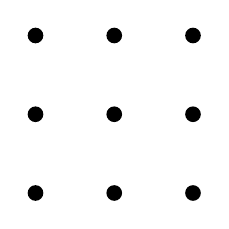
\begin{tikzpicture}
            \foreach \x in {0,1,2}
                \foreach \y in {0,1,2}
                    \draw (\x,\y) node[circle,fill,inner sep=2pt]{};
        \end{tikzpicture}
    };
    \node at ($(lattice.east) + (0.5,0)$) [right] {=};

    % Define combined structure with unit cell outline
    \node (crystal) at (8,0) {
        \begin{tikzpicture}
            % Draw unit cell outline
            \draw[black, thick] (0,0) rectangle (1,1);

            % Draw atoms
            \foreach \x in {0,1,2}
                \foreach \y in {0,1,2} {
                    \node[atom=blue] at (\x,\y) {};
                    \node[atom=red] at ($(\x,\y)+(0.5,0.5)$) {};
                }
        \end{tikzpicture}
    };

    % Labels
    \node at (motif.south) [below] {Motif/Basis};
    \node at (lattice.south) [below] {Point Lattice};
    \node at (crystal.south) [below] {Crystal Structure};

\end{tikzpicture}
\end{document}
